%UPDATEME%
The datasets used for this analysis are summarized in 
Tables.~\ref{tab:DatasetsData} and~\ref{tab:DatasetsMC} for data and Monte 
Carlo, respectively. The total integrated luminosity is 192 $\pm$ 8 $\ipb$. 
We used the official good run list~\cite{json}. For Monte Carlo simulation 
we use madgraph when possible, 
but different generators such as Pythia and Powheg 
are also used. 
For \wz\ and \zz\ processes we use Pythia, since MadGraph samples are mixed with $\WW$ in
a single $VV$ sample, which is difficult to use properly. 
For $gg \to \WW$ a dedicated generator is used. 


\begin{table}[!ht]
\begin{center}
\begin{tabular}{|c|c|}
\hline
 Dataset Description                   &   Dataset Name   \\
\hline
\hline
\multicolumn{2}{|c|}{$H \to \ZZ$ Signal Selection Samples} \\
\hline
Run2011A MuEl PromptReco            &  /MuEG/Run2011A-PromptReco-v*/AOD   \\
Run2011A DiMuon PromptReco          &  /DoubleMu/Run2011A-PromptReco-v*/AOD   \\
Run2011A SingleMuon PromptReco      &  /SingleMu/Run2011A-PromptReco-v*/AOD   \\
Run2011A DiElectron PromptReco      &  /DoubleElectron/Run2011A-PromptReco-v*/AOD   \\
\hline
\hline
\multicolumn{2}{|c|}{\fixme{}\bf Photon+Jets Samples} \\
\hline
Run2010A Jet  PromptReco            & /Jet/Run2011A-PromptReco-v*/AOD	\\
Run2010B Photon PromptReco          & /Photon/Run2011A-PromptReco-v*/AOD \\
\hline
\multicolumn{2}{|c|}{Fake Rate Measurement Samples} \\
\hline
Run2010A Jet  PromptReco            & /Jet/Run2011A-PromptReco-v*/AOD	\\
Run2010B Photon PromptReco          & /Photon/Run2011A-PromptReco-v*/AOD \\
\hline
\end{tabular}
\caption{Summary of data datasets used.}
\label{tab:DatasetsData}
\end{center}
\end{table}

\begin{table}[!ht]
\begin{center}
{\footnotesize
\begin{tabular}{|c|c|c|}
\hline
\multicolumn{3}{|c|}{With Pileup: Processed dataset name is always} \\
\multicolumn{3}{|c|}{/Spring11-PU\_S1\_START311\_V1G1-v*/AODSIM} \\
\hline
 Dataset Description                     &   Primary Dataset Name   & cross-section (pb)\\
\hline
qq $\rightarrow WW$                  	 &   /VVJetsTo4L\_TuneD6T\_7TeV-madgraph-tauola                        &  43.0  \\
gg $\rightarrow WW \to 2l 2\nu$          &   /GluGluToWWTo4L\_TuneZ2\_7TeV-gg2ww-pythia6                       &   0.153\\
$\ttbar$                              	 &   /TTJets\_TuneZ2\_7TeV-madgraph-tauola                             & 157.5 \\
$\singletops$                  	 	 &   /TToBLNu\_TuneZ2\_s-channel\_7TeV-madgraph                        &  1.4 \\
$\singletopt$                  	 	 &   /TToBLNu\_TuneZ2\_t-channel\_7TeV-madgraph                        &  20.9 \\
tW                                    	 &   /TToBLNu\_TuneZ2\_tW-channel\_7TeV-madgraph                       &  10.6 \\
Z[20-inf] $\rightarrow ee$	  	 &   /DYToEE\_M-20\_CT10\_TuneZ2\_7TeV-powheg-pythia                   &  1666.0 \\
Z[20-inf] $\rightarrow \mu\mu$        	 &   /DYToMuMu\_M-20\_CT10\_TuneZ2\_7TeV-powheg-pythia                 &  1666.0 \\	       
Z[20-inf] $\rightarrow \tau\tau$  	 &   /DYToTauTau\_M-20\_CT10\_TuneZ2\_7TeV-powheg-pythia-tauola        &  1666.0 \\
Z[10-20]  $\rightarrow ee$	  	 &   /DYToEE\_M-10To20\_CT10\_TuneZ2\_7TeV-powheg-pythia               &  3892.9 \\
Z[10-20]  $\rightarrow \mu\mu$    	 &   /DYToMuMu\_M-10To20\_CT10\_TuneZ2\_7TeV-powheg-pythia             &  3892.9 \\
Z[10-20]  $\rightarrow \tau\tau$  	 &   /DYToTauTau\_M-10To20\_CT10\_TuneZ2\_7TeV-powheg-pythia-tauola    &  3892.9 \\
W/Z+$\gamma$                       	 &   /PhotonVJets\_7TeV-madgraph                                       &  165.0 \\
W $\rightarrow$ $\ell\nu$           	 &   /WJetsToLNu\_TuneZ2\_7TeV-madgraph-tauola                         &  31314.0 \\
WZ                               	 &   /WZtoAnything\_TuneZ2\_7TeV-pythia6-tauola                        &  18.2 \\
ZZ                               	 &   /ZZtoAnything\_TuneZ2\_7TeV-pythia6-tauola                        &  7.4\\
$gg \to H \to ZZ \to 2\ell2\nu$          &   /GluGluToHToZZTo2L2Nu\_M-*\_7TeV-powheg-pythia6                   & vary \\
$gg \to H \to WW \to 2\ell2\nu$          &   /GluGluToHToWWTo2L2Nu\_M-*\_7TeV-powheg-pythia6                   & vary \\
$gg \to H \to WW \to \ell\tau2\nu$       &   /GluGluToHToWWTo2L2Nu\_M-*\_7TeV-powheg-pythia6                   & vary \\
$gg \to H \to WW \to 2\tau2\nu$          &   /GluGluToHToWWTo2Tau2Nu\_M-*\_7TeV-powheg-pythia6                 & vary \\
\hline
\hline
\end{tabular}
}
\caption{Summary of Monte Carlo datasets used.. The cross sections for a SM Higgs boson
is taken from the LHC Higgs cross-section working group~\cite{LHCHiggsCrossSectionWorkingGroup:2011ti}}
\label{tab:DatasetsMC}
\end{center}
\end{table}

Due to details in the implementation of the Powheg calculation in the Higgs MC, 
the Higgs $\pt$ spectrum for $gg \to H$ in MC has a much harder
spectrum compared with the most precise spectrum calculated to NNLO
with resummation to NNLL order, as illustrated in
Figure~\ref{fig:h160ww_pthiggs}{\fixme{}}. 
Therefore we reweight the MC simulated events according to the 
Higgs $\pt$ to match the spectrum obtained in NNLO calculation. 
This is done on the event-by-event level for both $gg \to H \to ZZ$ and 
$gg \to H \to WW$ processes. 
{\it\bf \fixme{} Add the details of ZZ pT reweighting.. }
 

%\begin{figure}[!htbp]
%\begin{center}
%   \subfigure[]{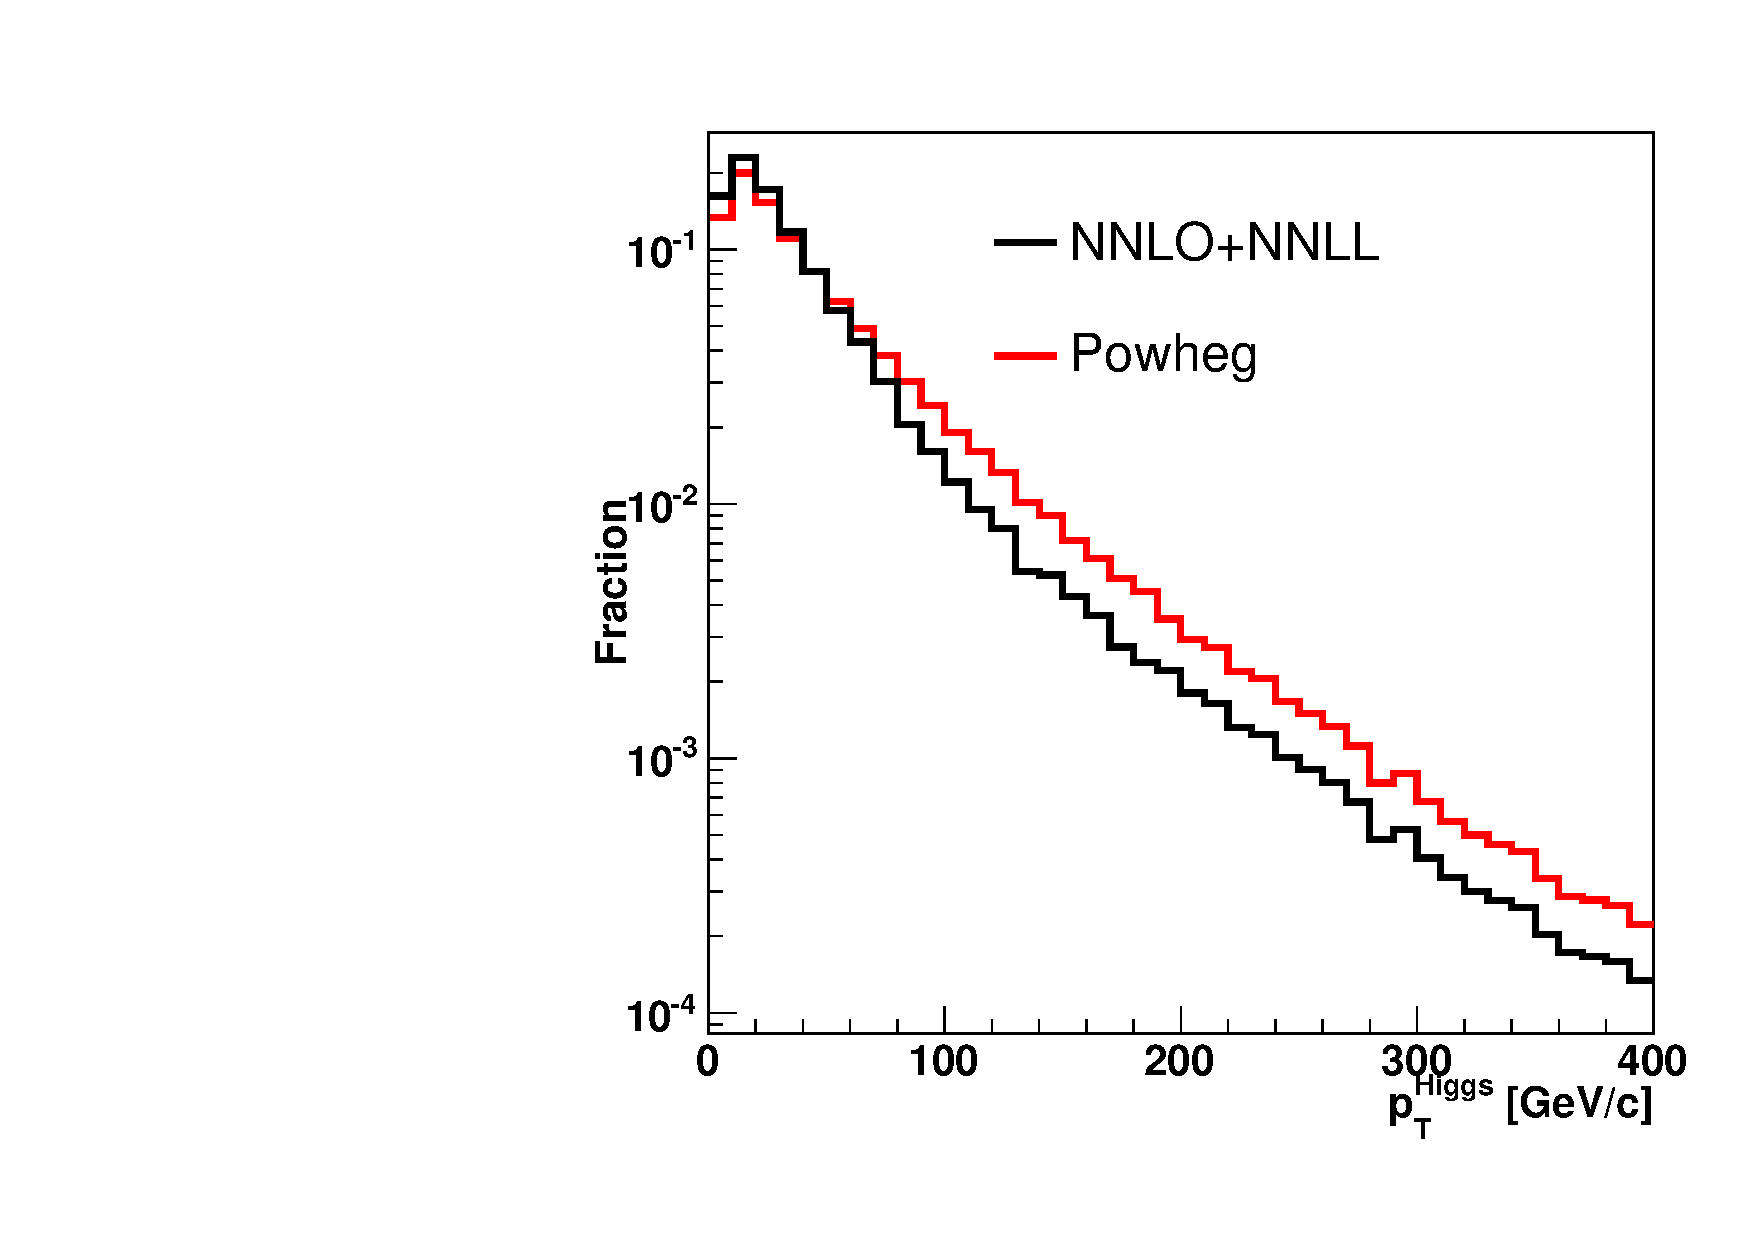
\includegraphics[width=0.49\textwidth]{figures/h160ww_pthiggs.pdf}}
%   \subfigure[]{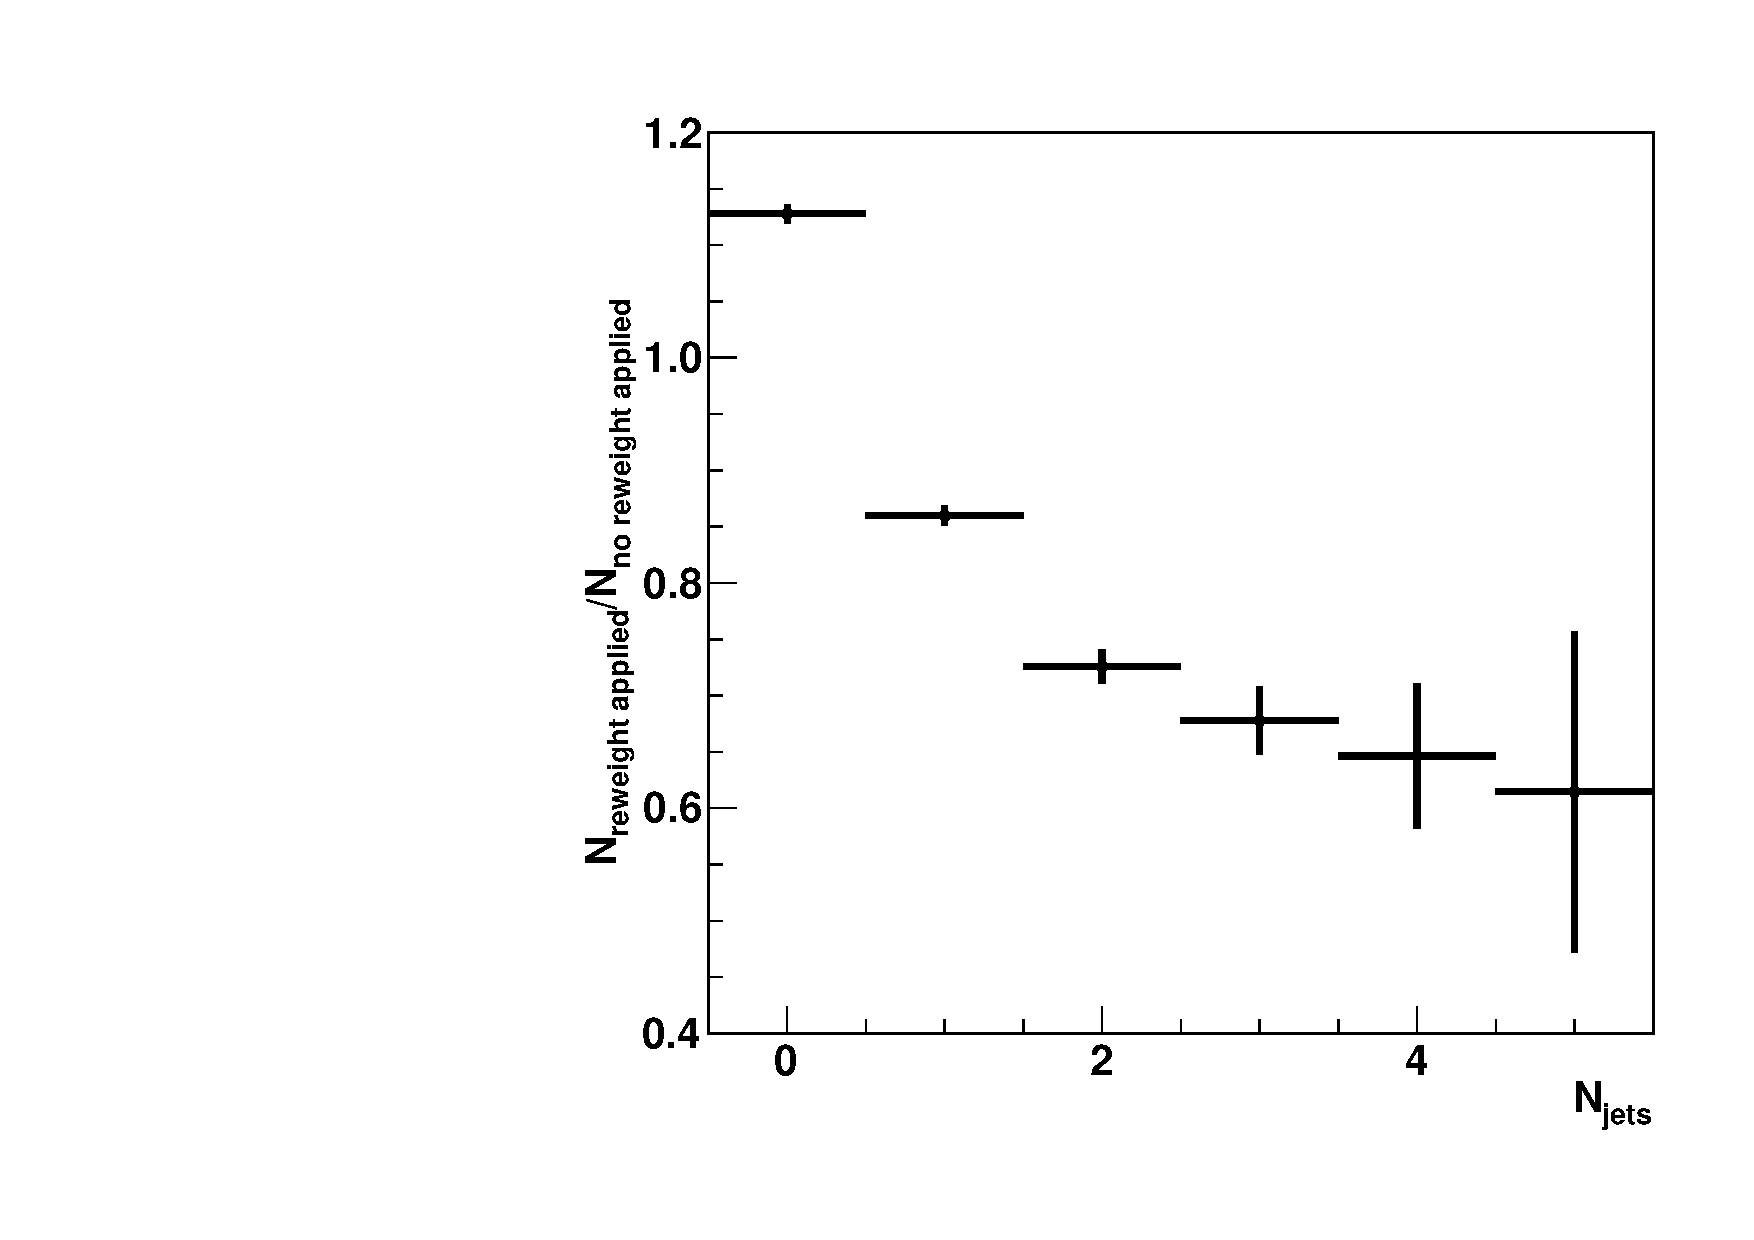
\includegraphics[width=0.49\textwidth]{figures/h160ww_njets_kfactor_ratio.pdf}} 
%\caption{(a) Higgs transverse momentum spectrum as predicted by Powheg and the NNLO+NNLL calculation; (b) 
%scale factors applied to each jet bin in the Powheg simulation.}
%\label{fig:h160ww_pthiggs}
%\end{center}
%\end{figure}
